\documentclass[11pt,a4paper]{article}
\usepackage[margin=1in]{geometry}
\usepackage[T1]{fontenc}
\usepackage{titlesec}
\usepackage{enumitem}
\usepackage{booktabs}
\usepackage{longtable}
\usepackage{xcolor}
\usepackage{fancyhdr}
\usepackage{hyperref}
\usepackage{parskip}
\usepackage{tikz}
\usetikzlibrary{positioning,arrows.meta}

\hypersetup{
  colorlinks=true,
  linkcolor=blue!60!black,
  urlcolor=blue!60!black,
  citecolor=blue!60!black
}

\pagestyle{fancy}
\fancyhf{}
\fancyhead[L]{PetSocial --- System Architecture}
\fancyfoot[C]{\thepage}
\renewcommand{\headrulewidth}{0.4pt}

\title{PetSocial\\\large System Architecture}
\author{PetSocial Development Documentation}
\date{\today}

\begin{document}
\maketitle
\thispagestyle{fancy}
\tableofcontents

\section{Technology Stack}

\begin{longtable}{@{}p{3.8cm}p{10.2cm}@{}}
\toprule
\textbf{Layer} & \textbf{Technology} \\
\midrule
\endhead
Framework & Next.js 16 (App Router), React 19, TypeScript \\
Styling & Tailwind CSS v4, a small shared component library
  (\texttt{Button}, \texttt{Card}, \texttt{Input}, \texttt{Avatar}, \texttt{Badge},
  \texttt{Icon}) \\
Database & PostgreSQL, hosted on Supabase \\
ORM & Prisma 7, using the \texttt{@prisma/adapter-pg} driver adapter over the
  \texttt{pg} client \\
Authentication & Supabase Auth (email/password), via \texttt{@supabase/ssr} for
  server-rendered session handling \\
File storage & Supabase Storage (a single \texttt{post-media} bucket, used for post
  photos, avatars, and listing photos) \\
Validation & Zod schemas in every server action \\
Rate limiting & A lightweight in-process, in-memory limiter (see
  \S\ref{sec:rate-limiting}) \\
Hosting & Vercel (application), Supabase (database, auth, storage) \\
\bottomrule
\end{longtable}

\section{High-Level Architecture}

PetSocial is a server-rendered application: the large majority of pages are React
Server Components that query the database directly through Prisma, and all writes go
through Next.js Server Actions rather than a separate REST or GraphQL API layer.

\begin{center}
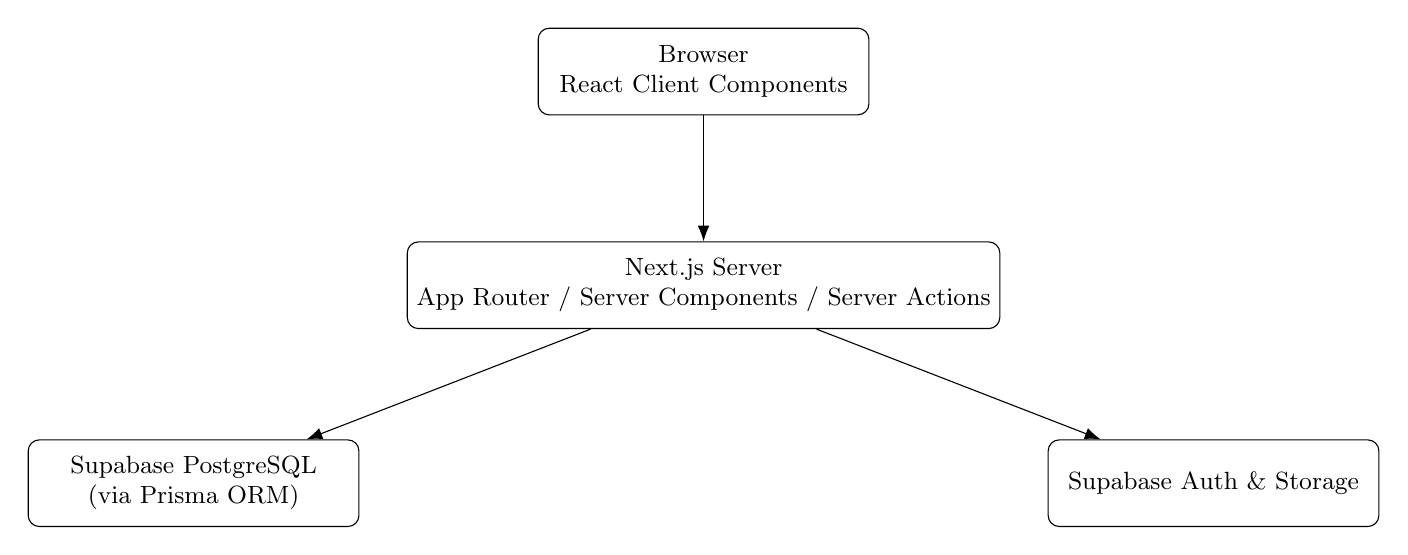
\begin{tikzpicture}[
  node distance=1.6cm and 2.2cm,
  box/.style={draw, rounded corners, align=center, minimum width=4.2cm,
              minimum height=1.1cm, font=\small}
]
\node[box] (client) {Browser\\React Client Components};
\node[box, below=of client] (server) {Next.js Server\\App Router / Server Components / Server Actions};
\node[box, below left=1.4cm and 0.6cm of server] (db) {Supabase PostgreSQL\\(via Prisma ORM)};
\node[box, below right=1.4cm and 0.6cm of server] (authstorage) {Supabase Auth \& Storage};

\draw[-{Latex[length=2mm]}] (client) -- (server);
\draw[-{Latex[length=2mm]}] (server) -- (db);
\draw[-{Latex[length=2mm]}] (server) -- (authstorage);
\end{tikzpicture}
\end{center}

\subsection{Request flow for a page view}
\begin{enumerate}[leftmargin=*]
  \item The browser requests a route (for example \texttt{/feed}).
  \item The corresponding \texttt{page.tsx} is a Server Component. It calls
        \texttt{createClient()} (a Supabase server client, see
        \texttt{src/utils/supabase/server.ts}) to read the current session from
        cookies, then queries Prisma directly for the data the page needs.
  \item The rendered HTML is streamed to the browser. Interactive pieces (forms, vote
        buttons, follow buttons) are separate, small Client Components.
\end{enumerate}

\subsection{Request flow for a mutation}
\begin{enumerate}[leftmargin=*]
  \item A form's \texttt{action} attribute is bound to a Server Action (a function
        marked \texttt{"use server"} in \texttt{src/app/actions/*.ts}), or a client
        component calls the action directly inside \texttt{useTransition} for
        button-triggered mutations (likes, follows, status toggles).
  \item The action re-derives the current user via \texttt{requireUser()}
        (\texttt{src/lib/auth.ts}), which redirects to \texttt{/login} if there is no
        session --- no page ever trusts a client-supplied user id.
  \item Input is parsed and validated with a Zod schema. On failure the action returns
        \texttt{\{ error: string \}}, which the calling Client Component renders inline.
  \item A per-user, per-action rate limit is checked via \texttt{rateLimit()}
        (\texttt{src/lib/rate-limit.ts}).
  \item The mutation is applied through Prisma. \texttt{revalidatePath()} marks the
        affected routes stale so the next render reflects the change.
\end{enumerate}

\section{Directory Structure}
\begin{longtable}{@{}p{4.5cm}p{9.5cm}@{}}
\toprule
\textbf{Path} & \textbf{Contents} \\
\midrule
\endhead
\texttt{src/app/*/page.tsx} & One folder per route, following the Next.js App Router
  convention. Dynamic segments use square brackets, e.g.\ \texttt{pets/[id]/page.tsx}. \\
\texttt{src/app/actions/*.ts} & Server Actions, grouped by feature area (one file per
  domain: \texttt{auth}, \texttt{pets}, \texttt{posts}, \texttt{engagement},
  \texttt{follows}, \texttt{lost-found}, \texttt{health}, \texttt{notifications},
  \texttt{messages}, \texttt{adoption}, \texttt{vet}, \texttt{marketplace},
  \texttt{profile}). \\
\texttt{src/components/} & Shared React components used across multiple pages
  (\texttt{Nav}, \texttt{BottomNav}, \texttt{Shell}, \texttt{PostCard},
  \texttt{VoteArrow}, \texttt{LeftSidebar}, \texttt{RightSidebar}). \\
\texttt{src/components/ui/} & Low-level, style-only primitives
  (\texttt{Button}, \texttt{Card}, \texttt{Input}, \texttt{Avatar}, \texttt{Badge},
  \texttt{Icon}, \texttt{EmptyState}). \\
\texttt{src/lib/} & Cross-cutting server utilities: \texttt{prisma.ts} (client
  singleton), \texttt{auth.ts} (\texttt{requireUser()}), \texttt{rate-limit.ts},
  \texttt{visibility.ts} (\texttt{isHidden()} anonymity helper), \texttt{notify.ts}
  (notification creation), \texttt{vet-seed.ts} (demo data seeding). \\
\texttt{src/utils/supabase/} & Three Supabase client constructors: \texttt{client.ts}
  (browser), \texttt{server.ts} (Server Components / Actions), \texttt{middleware.ts}
  (session refresh). \\
\texttt{src/generated/prisma/} & The generated Prisma Client. \textbf{Not committed to
  version control}; regenerated on every install via the \texttt{postinstall} script
  (see the Deployment Guide). \\
\texttt{prisma/schema.prisma} & The single source of truth for the data model. \\
\texttt{prisma/migrations/} & One directory per applied migration, in chronological
  order. \\
\bottomrule
\end{longtable}

\section{Session and Authentication Flow}
Supabase Auth issues a JWT session stored in cookies. Three separate Supabase client
constructors exist because each context has a different way of reading/writing those
cookies:

\begin{itemize}[leftmargin=*]
  \item \textbf{Browser client} (\texttt{utils/supabase/client.ts}) --- used inside
        Client Components, e.g.\ for direct-to-Storage file uploads.
  \item \textbf{Server client} (\texttt{utils/supabase/server.ts}) --- used inside
        Server Components and Server Actions; reads cookies via Next.js's
        \texttt{cookies()} API.
  \item \textbf{Middleware client} (\texttt{utils/supabase/middleware.ts}) --- runs on
        every request (\texttt{middleware.ts} at the project root) purely to refresh an
        expiring session before it reaches a Server Component.
\end{itemize}

\section{Rate Limiting}
\label{sec:rate-limiting}
Every mutating Server Action is rate-limited per user (keyed by user id and action
name) using an in-process \texttt{Map} of timestamps
(\texttt{src/lib/rate-limit.ts}). This is intentionally simple: it is correct for a
single running instance, but two important caveats apply:

\begin{itemize}[leftmargin=*]
  \item If the application is ever deployed across multiple serverless instances
        (which Vercel may do under load), each instance holds its own independent
        counters, so the effective limit is multiplied by the instance count.
  \item Counters are lost on every redeploy or cold start.
\end{itemize}

For a production deployment expected to receive meaningful traffic, this should be
replaced with a shared store (for example Upstash Redis) using the same
\texttt{rateLimit(key, limit, windowMs)} call signature, so no call sites need to
change.

\section{File Uploads}
All user-uploaded images (post photos, avatars, adoption/marketplace listing photos)
go directly from the browser to a single Supabase Storage bucket named
\texttt{post-media}, under feature-specific path prefixes (for example
\texttt{avatars/\{ownerId\}/...}, \texttt{adoption/\{ownerId\}/...},
\texttt{marketplace/\{ownerId\}/...}). Row-Level Security policies on the bucket permit
authenticated inserts and public reads; see the Security and Privacy document for the
exact policy definitions.

\end{document}
